\documentclass[a4paper,12pt]{scrartcl}
\usepackage[utf8x]{inputenc}
\usepackage[T1]{fontenc} % avec T1 comme option  d'encodage c'est ben mieux, surtout pour taper du français.
%\usepackage{lmodern,textcomp} % fortement conseillé pour les pdf. On peut mettre autre chose : kpfonts, fourier,...
\usepackage[french]{babel} %Sans ça les guillemets, amarchpo
\usepackage{amsmath}
\usepackage{multicol}
\usepackage{amssymb}
\usepackage{tkz-tab}
\usepackage{exercice_sheet}

%\trait
%\section*{}
%\exo{}
%\question{}
%\subquestion{}

\date{}


% Title Page
\title{Exercices : dérivées, $e$ et $\ln$}

\author{Mathématiques}

\begin{document}

\maketitle


\exo{}

\begin{figure}[h]
\begin{center}
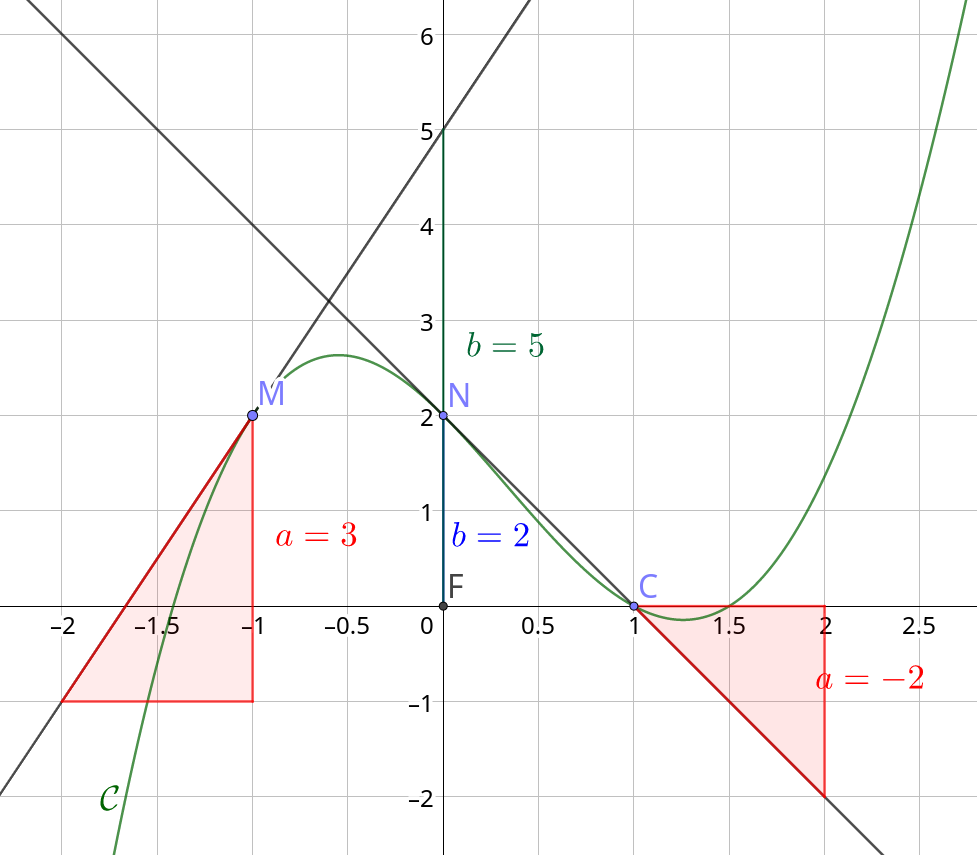
\includegraphics[width=0.8\textwidth]{pics/tangentes.png}
\end{center}
\end{figure}

\question{} 
\begin{itemize}
\item $f(-1)  = 2$
\item $f(0)   = 2$
\item $f(1)   = 0$
\item $f'(-1) = 3$
\item $f'(0)  = -2$
\end{itemize}

\question{Tangente en $M$:} 

Son coefficient directeur est $f'(-1) = 3$. Son ordonnée à l'origine est 5, par lecture graphique.

L'équation de la tangente en $M$ est donc $y = 3x+5$.

\question{Tangente en $N$:} 

Son coefficient directeur est $f'(-0) = -2$. Son ordonnée à l'origine est 2, par lecture graphique.

L'équation de la tangente en $M$ est donc $y = -2x+2$.

\exo{Calculs de dérivées}

\question{$f(x) = 5x^3-x^2+3x + \ln x - \dfrac{1}{x} + 4$}

\Answer{$f'(x) = 15 \, x^{2} - 2 \, x + \dfrac{1}{x} + \dfrac{1}{x^{2}} + 3$}

\question{$f(x) = 2 e^{-2x+1} - 5 \ln (3x+1)$}

\Answer{$f'(x) = -\dfrac{15}{3 \, x + 1} - 4 \, e^{-2 \, x + 1}$}

\question{$f(x) = (5x-1)e^{x}$}

$f$ est de la forme $u \times v$ avec:

$u(x) = 5x-1$ et $v(x) = e^{x}$, donc:

$u'(x) = 5$ et $v'(x) = e^{x}$.

$f' = u'v + uv'$ soit: 

$f'(x) = {\left(5 \, x - 1\right)} e^{x} + 5 \, e^{x}$, ce qui se factorise par $e^{x}$:

\Answer{$e^{x} \cdot (5x+4)$}

\question{$f(x) = \dfrac{1}{4x+1}$}

$f$ est de la forme $\dfrac{1}{u}$ avec:

$u(x) = 4x+1$, donc:

$u'(x) = 4$

$f' = \dfrac{-u'}{u^{2}}$ soit:


\Answer{$f'(x) = -\dfrac{4}{{\left(4 \, x + 1\right)}^{2}}$}

\question{$f(x) = \dfrac{e^{2x}}{3x+1}$}

\Answer{$\dfrac{{\left(6 \, x - 1\right)} e^{2 \, x}}{{\left(3 \, x + 1\right)}^{2}}$}

\question{$f(x) = (\ln x + 3)^{3}$}

On reconnaît ici que $f$ est de la forme $u^{\alpha}$ avec:

$u(x) = \ln x + 3$ et $\alpha = 3$

\Answer{$f'(x) = 3 \times \dfrac{1}{x} \times \, {\left(\ln x + 3\right)}^{2}$}

\question{$f(x) = \sqrt{4x+1} + \dfrac{1}{\sqrt{2x-1}}$}

Concernant $\dfrac{1}{\sqrt{2x-1}}$: elle est de la forme $\dfrac{1}{u}$ avec $u(x) = \sqrt{2x-1}$. 

$u$ est elle-même une composée: $u = v \circ w$ avec $v(x) = \sqrt{x}$ et $w(x) = 2x-1$.

On a donc $u'(x) = w'(x) \times v'(w(x))$. 

Donc $u'(x) = \dfrac{2}{2\sqrt{2x-1}} = \dfrac{1}{\sqrt{2x-1}}$.

Or, la dérivée de la forme $\dfrac{1}{u}$ est $\dfrac{-u'}{u^{2}}$.

On a donc $\left(\dfrac{1}{\sqrt{2x-1}}\right)' = - \dfrac{1}{\left(2 \, x - 1\right) \sqrt{2 \, x - 1}}$

\Answer{$f'(x) = \dfrac{2}{\sqrt{4 \, x + 1}} - \dfrac{1}{\left(2 \, x - 1\right) \sqrt{2 \, x - 1}}$}



\question{$f(x) = \sin(2x+1) + \cos x^2$ (hors programme en CG)}

\Answer{$f'(x) = 2 \, \cos\left(2 \, x + 1\right) -2 \, x \sin\left(x^{2}\right)$}

\exo{}

\question{$3^{x} = 2$}

$\Leftrightarrow \ln(3^{x}) = \ln 2$

$\Leftrightarrow x \ln 3 = \ln 2$

$\Leftrightarrow x  = \dfrac{\ln 2}{\ln 3}$

\Answer{$\mathcal{S} = \left\lbrace \dfrac{\ln 2}{\ln 3} \right\rbrace$}

\question{$3 \times 5^{x} + 8 = 9$}

$\Leftrightarrow  = 3 \times 5^{x} = 1$

$\Leftrightarrow  = 5^{x} = \dfrac{1}{3}$

$\Leftrightarrow  = \ln \left( 5^{x}\right) = \ln \left( \dfrac{1}{3}\right)$

$\Leftrightarrow  = x \ln \left( 5\right) = - \ln \left( 3\right)$

\Answer{$\mathcal{S} = \left\lbrace -\dfrac{\ln 3}{\ln 5}\right\rbrace$}

\question{$3 \times 4^{2x+1} = 6$}

$\Leftrightarrow 4^{2x+1} = 2$

$\Leftrightarrow \ln \left( 4^{2x+1} \right) = \ln 2$

$\Leftrightarrow (2x+1) \ln 4 = \ln 2$

$\Leftrightarrow (2x+1) \ln 4 = \ln 2$

$\Leftrightarrow 2x+1 = \dfrac{\ln 2}{\ln 4}$

$\Leftrightarrow 2x+1 = \dfrac{1}{2}$

$\Leftrightarrow x = -\dfrac{1}{4}$

\Answer{$\mathcal{S} = \left\lbrace -\dfrac{1}{4} \right\rbrace$}

\question{$3 e^{x} - 1 = 5$}

$\Leftrightarrow e^{x} = 2$

$\Leftrightarrow x = \ln 2$

\Answer{$\mathcal{S} = \left\lbrace \ln 2 \right\rbrace$}

\question{$e^{x^{2}} = 4$}

$\Leftrightarrow x^{2} = \ln 4$

$\Leftrightarrow x = \sqrt{\ln 4}$ ou $x = -\sqrt{\ln 4}$

\Answer{$\mathcal{S} = \left\lbrace -\sqrt{\ln 4} ; \sqrt{\ln 4} \right\rbrace$}

\exo{}

\question{$\ln(3x) = 4$}

$\Leftrightarrow e^{\ln(3x)} = e^{4}$

$\Leftrightarrow x = \dfrac{e^{4}}{3} $

\Answer{$\mathcal{S} = \left\lbrace \dfrac{e^{4}}{3} \right\rbrace$}

\question{$2 \ln(4x + 1) = 4$}

$\Leftrightarrow \ln(4x + 1) = 2$

$\Leftrightarrow 4x + 1 = e^2$

$\Leftrightarrow x = \dfrac{e^2 - 1}{4}$

\Answer{$\mathcal{S} = \left\lbrace \dfrac{e^2 - 1}{4} \right\rbrace$}

\question{$5-3 \ln x = 8$}

$\Leftrightarrow \ln x = -1$

$\Leftrightarrow x = e^{-1} = \dfrac{1}{e}$

\Answer{$\mathcal{S} = \left\lbrace \dfrac{1}{e} \right\rbrace$}

\exo{Résoudre les inéquations}

\question{$5^{x} > 4$}

$\Leftrightarrow \ln(5^{x}) > \ln 4$

$\Leftrightarrow x \ln 5 > \ln 4$

$\Leftrightarrow x > \dfrac{\ln 4}{\ln 5}$ (l'inégalité ne change pas de sens car $\ln 5 > 0$).

\Answer{$\mathcal{S} = \left] \dfrac{\ln 4}{\ln 5} ; +\infty \right[$}

\question{$0.8^{x} < 3$}

$\Leftrightarrow x > \dfrac{\ln 3}{\ln 0.8}$ car $\ln 0.8 < 0$.

\Answer{$\mathcal{S} = \left] \dfrac{\ln 3}{\ln 0.8} ; +\infty \right[$}

\exo{}

D'après l'énoncé, on a $\ln z = 2x+1$. 

$\Leftrightarrow z = e^{2x+1}$

Soit $z = e \times e^{2x} \approx 2.7 \times e^{2x}$.

On a donc $k \approx 2.7$ et $\lambda = 2$

\exo{}

$(2x+1)^{3} = e^{y}$

$\Leftrightarrow y = \ln \left( (2x+1)^{3} \right)$

$y = 3 \ln(2x+1)$

$y$ s'écrit donc bien de la forme $A \ln(2x+1)$ avec $A = 3$.

\exo{}

$\ln \left( \dfrac{v-2}{t-5} \right) = -t+3$

\question{}

$\ln \left( \dfrac{v-2}{t-5} \right) = -t+3$

$\Leftrightarrow \dfrac{v-2}{t-5} = e^{-t+3}$

$\Leftrightarrow v = (t-5)e^{-t+3} + 2$

$\Leftrightarrow v = e^{3}(t-5)e^{-t} + 2$

On a donc $v = \alpha (t-5) e^{\beta t} + \theta$ avec \answer{$\alpha \approx 20.1$, $\beta = -1$ et $\theta = 2$}

\question{}

Pour $t = 6.3$: 

$v = 20.1 \times (6.3-5)e^{-6.3} + 2$

\Answer{$v \approx 2.048$}


\trait

\end{document}



%\question{$•$}
%
%
%
%\Answer{$\mathcal{S} = \left\lbrace  \right\rbrace$}
